% Provenance (never printed): see sources/outline_sources.md (Year 2: the long-term carbon cycle
% and the silicate-weathering thermostat; Palaeozoic glaciations; the Cretaceous greenhouse; the
% PETM; Cenozoic cooling). Reservoirs from IPCC AR6 WG1 Figure 5.12; long-term fluxes after Derry
% (2024); weathering laws after Colbourn and others (2013); Phanerozoic CO2 after Foster and
% others (2017); Phanerozoic temperatures after Judd and others (2024); Cenozoic isotopes from
% CENOGRID (Westerhold 2020); the Eocene--Oligocene transition after Hutchinson and others (2021);
% the PETM after AR6 WG1 chapters 2 and 5. The thermostat model, its curves and every number of
% the exercises and problem from figdata/bachelor-2/deeptime.py and the Book 4 second-writer
% scratch calculator calc/ch26.py.
\chapter{地质时期的气候}\label{ch:b2:deep-time-climate}

五千万年前，地球上任何地方都没有冰盖。大气中二氧化碳含量超过
百万分之一千，两极的升温远大于赤道，而接近热带类型的森林生长在
南纬 \ang{70} 处，经历整个极夜期。三千四百万年前，
冰覆盖了南极洲，此后再未消失。岩层所记录的数亿年间，
地球在有冰与无冰的世界之间来回摆动；然而自
雪球事件（见
\cref{ch:b2:precambrian-earth}）以来，它从未将海洋烧干，也从未永久冻结。本章讨论决定这些气候的碳，
它在大气与岩石之间缓慢循环，以及使行星
保持宜居的恒温机制。
% ledger: ipcc:ref-periods, ar6ch2:cenozoic, hutchinson21:eot

\begin{recall}
\textbf{中学分册内容}：温室效应与辐射强迫；
二氧化碳的强迫随其浓度的对数增长，倍增时为 \qty{3.93}{W.m^{-2}}；
平衡气候敏感度，最佳估计 \qty{3}{\celsius}；脱气；\omterm{def:b2:orbital-forcing:glacials}{冰期}旋回
与末次盛\omterm{def:b2:orbital-forcing:glacials}{冰期}。\textbf{本科一年级分册内容}：化学风化与
硅酸盐的水解；黏土矿物；碳酸盐软泥、溶跃面与碳酸盐
补偿深度。\textbf{前文内容}：暗淡的年轻太阳与\omterm{def:b2:precambrian-earth:snowball}{雪球地球}
（\cref{ch:b2:precambrian-earth}）；\omterm{def:b2:phanerozoic-earth:palaeogeography}{古地理学}与\omterm{def:b2:phanerozoic-earth:oae}{大洋缺氧事件}
（\cref{ch:b2:phanerozoic-earth}）；\omterm{def:b2:climate-proxies:proxy}{气候代用指标}、$\delta^{18}$O 与\omterm{def:b2:climate-proxies:ice-volume}{冰量效应}
（\cref{ch:b2:climate-proxies}）；轨道强迫（\cref{ch:b2:orbital-forcing}）。碳循环、
其储库与停留时间属于生物学分册，
阿伦尼乌斯定律属于化学分册。
\end{recall}
% ledger: ipcc:erf-2xco2, ipcc:log-co2, ipcc:ecs

\section{长期碳循环}\label{sec:b2:deep-time-climate:cycle}

\subsection*{储库与通量}

\begin{definition}[长期碳循环；碳酸盐–硅酸盐循环]\label{def:b2:deep-time-climate:carbon-cycle}
\emph{长期碳循环}\index{长期碳循环}是表层储库（大气、海洋、生物圈与土壤）
与固体地球之间的碳交换：火山与变质脱气、岩石风化，
以及碳酸盐与有机碳在沉积物中的埋藏。这些沉积物
随后转变为岩石或被俯冲。其通量相对表层储库很小，
作用时间尺度为 $10^5$ 至 $10^8$ 年。其无机部分为
\emph{碳酸盐–硅酸盐循环}\index{碳酸盐–硅酸盐循环}：二氧化碳从地幔与地壳中在火山处逸出，
被硅酸盐岩石的风化所消耗，以碳酸盐形式沉积于海底，
当该碳酸盐发生变质或俯冲脱气时，
重新返回表层。
\end{definition}
% ledger: derry24:fluxes, derry24:subduction, colbourn13:timescale

生物学分册沿光合作用、呼吸作用与海洋追踪碳的去向，时间尺度从数年
到数百年。在气候史的时间尺度上，图景还要扩展到岩石。工业化以前，
大气中含有 \qty{591}{PgC}（拍克碳，即十亿吨碳）；
海洋含有 \num{38700}，其中几乎全部为中层与深层水中的溶解无机碳（\num{37100}）；
植被、土壤与永久冻土合计含有 \num{3350}。活跃的表层储库合计约含
\num{3.5e6} 太摩尔碳，约合 \qty{42000}{PgC}。沉积岩中也含有碳，
以石灰岩的形式存在，也以分散于页岩中的有机质形式存在，
它们与表层的交换十分缓慢。
% ledger: ar6ch5:fig512, derry24:residence

据现代估算，碳的输入与输出（单位为每年太摩尔碳，$\qty{1}{Tmol}$ 碳等于
\qty{0.012}{PgC}）如下。进入海洋与大气的部分：洋中脊火山脱气（1.3）、洋岛（1.3）、
岛弧（4.5）与大陆裂谷（4.2），合计约 11；变质脱气为 2 至 4；老碳酸盐的风化为 12.3，
由侵蚀暴露的老有机碳氧化为 8.1，另有地质甲烷 2.0，合计 \num{36.7}。
输出的部分：碳酸盐沉积约 26，有机碳埋藏约 16。
两侧在各自的不确定度范围内平衡。地球内部脱气提供的输入
略多于三分之一（见\cref{exo:b2:deep-time-climate:2}）；
其余为沉积碳的再次循环。
其他估算给出的火山通量更低：全球碳预算（IPCC）中为每年
\qty{0.1}{PgC}（约 8 Tmol）；美国地质调查局的一项调查中为
\qty{0.26}{Gt} 二氧化碳（约 6 Tmol 碳）。
火山输入的不确定度约为二倍。
% ledger: derry24:fluxes, ar6ch5:fig512, usgs:volcanic-co2

\begin{omfigure}
\centering
\begin{tikzpicture}[font=\scriptsize, >={Stealth[length=2mm]},
  box/.style={draw, thick, rounded corners=2pt, align=center, inner sep=4pt},
  up/.style={->, very thick, omThm}, down/.style={<-, very thick, omDef},
  lab/.style={midway, above, sloped, font=\scriptsize}]
% reservoirs: ar6ch5:fig512; active reservoirs derry24:residence; fluxes derry24:fluxes, derry24:subduction
\draw[thick, rounded corners=2pt, fill=blue!6] (-6.3,0) rectangle (6.0,2.6);
\node[anchor=north west, font=\small\bfseries] at (-6.2,2.55) {表层储库，约 \qty{42000}{PgC}};
\node[box, fill=white] (atm) at (-4.6,1.45) {大气 \\\qty{591}{PgC}};
\node[box, fill=white] (oc) at (0.6,1.45) {海洋 \\\qty{38700}{PgC}};
\node[box, fill=white] (land) at (4.3,1.45) {植被、土壤、\\永久冻土 \qty{3350}{PgC}};
\draw[->, very thick, omProp] (atm.east) -- (oc.west);
\node[align=center, text=omProp] at (-2.0,0.6) {硅酸盐风化 11--12，以碳酸氢盐形式};
\draw[<->, thick, black!50] (oc.east) -- (land.west);
% sedimentary rocks and mantle
\node[box, fill=brown!12, minimum width=5.7cm, minimum height=1.1cm] (rock) at (-3.35,-4.55) {沉积岩：\\碳酸盐与有机碳};
\node[box, fill=orange!15, minimum width=3.0cm, minimum height=1.1cm] (mantle) at (4.3,-4.55) {地幔};
% inputs (red, up) and outputs (blue, drawn upwards with the tip at the start)
\draw[up] (-5.7,-4.0) -- node[lab] {碳酸盐风化 12.3} (-5.7,0);
\draw[up] (-4.8,-4.0) -- node[lab] {老有机碳氧化 8.1} (-4.8,0);
\draw[up] (-3.9,-4.0) -- node[lab] {地质甲烷 2.0} (-3.9,0);
\draw[up] (-3.0,-4.0) -- node[lab] {变质脱气 2--4} (-3.0,0);
\draw[down] (-1.9,-4.0) -- node[lab] {碳酸盐沉积 26} (-1.9,0);
\draw[down] (-1.0,-4.0) -- node[lab] {有机碳埋藏 16} (-1.0,0);
\draw[up] (4.3,-4.0) -- node[lab] {火山与裂谷 11.3} (4.3,0);
\draw[->, very thick, black!70] (rock.east) -- node[above] {俯冲 4--6} (mantle.west);
\end{tikzpicture}
\par\smallskip{\small \omterm{def:b2:deep-time-climate:carbon-cycle}{长期碳循环}图，工业化以前的储库数据取自 IPCC
全球碳预算，现今通量取自 2024 年的一项综合研究，单位为每年太摩尔碳
（\qty{1}{Tmol.\text{年}^{-1}} = \qty{0.012}{PgC.\text{年}^{-1}}）。红色：输入表层储库；蓝色：
输出。硅酸盐风化并不离开表层：它将碳从大气以碳酸氢盐形式转入
海洋，之后以碳酸盐沉积物的形式离开。}
\end{omfigure}

用通过它们的通量去除地表储库的 \qty{3.5e6}{Tmol}，
得到碳的停留时间为 8 至 \num{9e4} 年。进入海洋和大气的碳
会在约数十万年内再次被埋藏，以本章的尺度看只是一瞬间：地表
储库紧随缓慢的输入与输出变化，二者之间任何持续的失衡
都会改变大气中的二氧化碳含量。
% ledger: derry24:residence

\subsection*{碳酸盐与硅酸盐风化}

雨水溶解二氧化碳并侵蚀岩石，正如本科一年级分册所述。两类岩石的
行为差别很大。风化一块石灰岩时，从大气中取走一个二氧化碳，同时
把岩石中的一个碳带入水中；海洋生物用这些产物构筑外壳时，
又有一个碳回到大气中：
\[
  \ce{CaCO3 + CO2 + H2O -> Ca^{2+} + 2 HCO3^-} , \qquad
  \ce{Ca^{2+} + 2 HCO3^- -> CaCO3 + CO2 + H2O} .
\]
石灰岩的往返过程对大气的净效应为零。硅酸盐风化，此处以硅灰石作为
花岗岩和玄武岩中钙硅酸盐的代表，同样消耗二氧化碳，
但不从岩石中带来任何碳：
\[
  \ce{CaSiO3 + 2 CO2 + H2O -> Ca^{2+} + 2 HCO3^- + SiO2} ,
\]
由其生成的碳酸盐只归还两者中的一个：
\[
  \ce{CaSiO3 + CO2 -> CaCO3 + SiO2} \quad\text{（净）} .
\]
因此，陆地上每风化一摩尔钙或镁硅酸盐，便有一摩尔二氧化碳
锁入碳酸盐岩中。这正是碳酸盐沉积（约 26）超过碳酸盐风化
（12.3）的原因，其差额大致等于硅酸盐风化每年消耗的 11 至 12 太摩尔；而
正是硅酸盐风化而非碳酸盐风化，在数百万年的尺度上与火山释放相平衡。
% ledger: colbourn13:timescale, derry24:fluxes

\section{硅酸盐风化恒温器}\label{sec:b2:deep-time-climate:thermostat}

\subsection*{负反馈}

硅酸盐风化是一种化学反应，与多数化学反应一样，温度升高时反应更快。温暖
还会带来更多降雨与径流，它们将产物带走，并把新鲜水输送到
岩石表面。因此风化速率随温度升高而增大；温度则随大气二氧化碳
含量的增加而升高。一颗获得更多二氧化碳的行星会变暖、风化加快，随后又失去这些二氧化碳。

\begin{definition}[硅酸盐风化恒温器]\label{def:b2:deep-time-climate:thermostat}
\emph{硅酸盐风化恒温器}\index{硅酸盐风化恒温器}是气候与\omterm{def:b2:deep-time-climate:carbon-cycle}{长期碳循环}之间的
负反馈：硅酸盐岩石的风化将二氧化碳从大气移入碳酸盐岩，
其速率随温度和径流增大，因此大气二氧化碳含量升高会提高自身的移除速率，
含量降低则使移除速率随之减小。在 $10^5$ 至 $10^6$ 年的时间内，它使移除量
重新与脱气量达到
平衡。
\end{definition}
% ledger: colbourn13:timescale, colbourn13:weathering, hutchinson21:gateways

温度依赖关系即化学书中的阿伦尼乌斯定律。设硅酸盐中钙和镁溶解的
活化能为 $E_{\text a}$，则风化通量在
温度 $T$ 接近参考温度 $T_0$ 时为
\[
  W = W_0 \exp\Bigl[-\frac{E_{\text a}}{R}\Bigl(\frac1T - \frac1{T_0}\Bigr)\Bigr]
  \approx W_0\, e^{k_T (T - T_0)}, \qquad k_T = \frac{E_{\text a}}{R T_0^2},
\]
由于 $1/T - 1/T_0 \approx -(T - T_0)/T_0^2$。实验室溶解测得 $E_{\text a} =
\qty{63}{kJ.mol^{-1}}$，取 $T_0 = \qty{288}{K}$，则 $k_T = \qty{0.09}{K^{-1}}$：温度每升高一度，
通量约增加 \qty{9}{\percent}；在 $T_0$ 上下十度范围内，近似与精确定律
的偏差小于 \qty{3}{\percent}（见\cref{exo:b2:deep-time-climate:6}）。现场估计为
$74 \pm \qty{29}{kJ.mol^{-1}}$，因此灵敏度的不确定度约为两倍。径流
的影响也会叠加：取通量正比于 $(R/R_0)^{0.65}$，且径流
每升高一度增加 \qty{4.5}{\percent}，则综合灵敏度为 $k = 0.09 + 0.65\times0.045 =
\qty{0.119}{K^{-1}}$。
% ledger: colbourn13:weathering
% values: k_run 0.11925 (deeptime.py)

\subsection*{单箱模型}

要看恒温器的响应有多快，需追踪海洋与大气所含的
高于稳态的过量碳 $M$。扰动发生后的数千年内，海洋和海底碳酸盐
已从大气中移走了过量碳的大部分；若释放 \qty{4000}{PgC}，约
\qty{8}{\percent} 留在大气中，直到硅酸盐风化将其移除。记 $f$ 为
该比例，$A_0 = \qty{591}{PgC}$ 为大气的工业化以前碳含量，于是大气二氧化碳含量
为 $C = C_0(1 + fM/A_0)$。变暖遵循对数律，气候灵敏度为
$S$，$\Delta T = S\log_2(C/C_0)$，风化则遵循上述指数律。
% ledger: colbourn13:timescale, ar6ch5:fig512, ipcc:ecs, ipcc:log-co2

\begin{proposition}[恒温器的稳态与时间常数]\label{prop:b2:deep-time-climate:thermostat}
设海洋–大气的过量碳 $M$ 按下式变化：
\[
  \frac{\mathrm dM}{\mathrm dt} = V - W_0\,e^{k\,\Delta T(M)}, \qquad
  \Delta T(M) = S\log_2\Bigl(1 + \frac{fM}{A_0}\Bigr),
\]
其中 $V$ 为脱气量，$W_0$ 为 $M = 0$ 时的风化量。
\begin{enumerate}
  \item 稳态时 $\Delta T^* = \ln(V/W_0)/k$，与 $S$ 和 $f$ 无关。
  \item 若 $V = W_0$，则小的过量按 $M(t) = M(0)\,e^{-t/\tau}$ 衰减，其中
        \[
          \tau = \frac{A_0 \ln 2}{f\,k\,S\,W_0} .
        \]
\end{enumerate}
\end{proposition}

\begin{proof}
(1) 稳态时 $\mathrm dM/\mathrm dt = 0$，故 $W_0e^{k\Delta T^*} = V$，$\Delta T^* =
\ln(V/W_0)/k$；$S$ 与 $f$ 均不出现。(2) 在 $M = 0$ 附近，$\log_2(1 + x) \approx x/\ln 2$，于是
$\Delta T \approx SfM/(A_0\ln 2)$，$e^{k\Delta T} \approx 1 + kSfM/(A_0\ln2)$。当 $V = W_0$ 时，
方程化为 $\mathrm dM/\mathrm dt = -W_0kSfM/(A_0\ln 2) = -M/\tau$，其解即为
指数函数。
\end{proof}

第一条结论是恒温器的核心。它固定的是温度而非浓度：若火山脱气增加
\qty{20}{\percent}，地球最终稳定在比原先高 $\ln 1.2/0.09 = \qty{2.0}{\celsius}$ 的
温度，与其气候灵敏度无关；二氧化碳则会调整到能产生这一增温的水平，
即增加 \qty{60}{\percent}。风化响应弱、$k$ 小，是较差的恒温器；
响应强的则能将温度几乎固定。
% values: dT_step 2.026, C_step_ratio 1.597 (deeptime.py)

\begin{example}[恒温器的时间常数]\label{ex:b2:deep-time-climate:tau}
硅酸盐风化每年消耗 11 至 \qty{12}{Tmol} 的碳；取 $W_0 = 11.5\times0.012011
= \qty{0.138}{PgC.\text{年}^{-1}}$。取 $A_0 = \qty{591}{PgC}$，$f = 0.08$，$k = \qty{0.09}{K^{-1}}$ 和
$S = \qty{3}{K}$，则
\[
  \tau = \frac{591\times0.693}{0.08\times0.09\times3\times0.138} = \qty{1.37e5}{\text{年}} ,
\]
约 14 万年。若计入径流因子，取 $k = 0.119$，则缩短为
\qty{104}{ka}。
\end{example}
% ledger: derry24:fluxes, ar6ch5:fig512, colbourn13:timescale, colbourn13:weathering, ipcc:ecs
% values: tau_kT_kyr 137.3, tau_run_kyr 103.6 (deeptime.py)

模型较为粗略：比例 $f$ 并非常数，海洋化学被简化为一个
数，风化也简化为一条全球规律。显式包含海洋与沉积物的模型给出
的 e 折时间约为 \qty{200}{ka} 至一百万年。因此，恒温器是
极长时间尺度上的调节器：它对未来几千年的气候毫无影响，而
它能将地球温度在数亿年间维持在一定范围之内。
% ledger: colbourn13:timescale

\begin{omfigure}
\centering
\begin{tikzpicture}
\begin{groupplot}[group style={group size=2 by 1, horizontal sep=1.6cm},
  omrecord, width=0.47\linewidth, height=5.4cm, xmin=0, xmax=1000,
  xlabel={时间 (\unit{ka})}, xtick pos=bottom, ytick pos=left,
  tick label style={font=\scriptsize}, label style={font=\small},
  legend style={draw=none, fill=white, font=\scriptsize}]
\nextgroupplot[ymin=0, ymax=5200, ylabel={过剩碳 (\unit{PgC})},
  y tick label style={/pgf/number format/1000 sep={\,}},
  legend style={at={(0.97,0.97)}, anchor=north east}]
% computed in figdata/bachelor-2/deeptime.py part pulse; ledger: colbourn13:timescale, colbourn13:weathering, derry24:fluxes, ar6ch5:fig512, ipcc:ecs
\addplot[omThm, line width=1.2pt] table[x=t_kyr, y=M_nl] {figdata/out/bachelor-2-deeptime-pulse.dat};
\addlegendentry{模型}
\addplot[black, densely dashed, line width=1.0pt] table[x=t_kyr, y=M_lin] {figdata/out/bachelor-2-deeptime-pulse.dat};
\addlegendentry{线性化}
\draw[densely dotted] (axis cs:137.3,0) -- (axis cs:137.3,1839);
\node[anchor=west, font=\scriptsize] at (axis cs:145,1400) {$\tau$};
\nextgroupplot[ymin=0, ymax=2.4, ylabel={增温 (\unit{\celsius})},
  legend style={at={(0.97,0.03)}, anchor=south east}]
% computed in figdata/bachelor-2/deeptime.py part step
\addplot[omThm, line width=1.2pt] table[x=t_kyr, y=dT_nl] {figdata/out/bachelor-2-deeptime-step.dat};
\addlegendentry{模型}
\addplot[black, densely dashed, line width=1.0pt] table[x=t_kyr, y=dT_lin] {figdata/out/bachelor-2-deeptime-step.dat};
\addlegendentry{线性化}
\draw[densely dotted] (axis cs:0,2.026) -- (axis cs:1000,2.026);
\node[anchor=south east, font=\scriptsize] at (axis cs:1000,2.03) {$\ln 1.2/k$};
\end{groupplot}
\end{tikzpicture}
\par\smallskip{\small 单箱恒温器，取 $k = \qty{0.09}{K^{-1}}$ 和 $S = \qty{3}{K}$。
左图：零时刻释放 \qty{5000}{PgC}，计量时已扣除海洋与碳酸盐所占的
份额；其按 e 折时间 $\tau$ 衰减，起初略慢于
线性化规律。右图：零时刻脱气量增加 \qty{20}{\percent}，地球
逐渐升温，趋向 \cref{prop:b2:deep-time-climate:thermostat} 所给的稳定增温 \qty{2.0}{\celsius}。}
\end{omfigure}
% values: t90_lin_kyr 316.2, t90_nl_kyr 339.9, tau_step_kyr 182.7 (deeptime.py)

恒温器还可解释\cref{ch:b2:precambrian-earth}中提到的弱年轻太阳问题。太阳亮度
每隔数亿年增强几个百分点，若空气成分固定，地球便随之升温；
但温度升高意味着风化加快，从而拉低二氧化碳含量，直至温度
回落到接近脱气所决定的水平。过去 4.2 亿年的岩石记录恰好印证了这一点，
如下一节所述。

\section{温室世界与冰室世界}\label{sec:b2:deep-time-climate:states}

\begin{definition}[温室气候状态与冰室气候状态]\label{def:b2:deep-time-climate:states}
称\emph{温室气候状态}\index{温室气候状态}为一段持续数百万至
数千万年的长时期，其间无大陆冰盖，大气二氧化碳含量高，
赤道与两极之间的温差小。称\emph{冰室气候状态}\index{冰室气候状态}为一段
长时期，其间一极或两极存在大陆冰盖，
二氧化碳含量较低，赤道至两极的梯度陡峭。地球自
约 \qty{34}{Ma} 以来处于冰室状态。
\end{definition}
% ledger: judd24:phanda, hutchinson21:eot

\subsection*{过去 4.2 亿年的二氧化碳}

冰芯出现以前的二氧化碳含量由代用指标读取，包括硼同位素和
海洋浮游生物的有机分子、化石叶片的孔隙、古土壤中的碳酸盐结核。2017 年的一项汇编
将这些数据平滑后回溯至 \qty{420}{Ma}，并与\omterm{def:b2:orbital-forcing:glacials}{冰期}一同示于下方。其
长期趋势为每百万年约下降 \qty{3.4}{ppm}，接近工业化前水平的数值
在我们所处时代之前共出现两次：石炭纪和二叠纪，以及
晚白垩世的短暂时期。
% ledger: foster17:co2, data:b4-foster2017, ar6ch2:deep-co2

\begin{omfigure}
\centering
\begin{tikzpicture}
\begin{axis}[omrecord, omage, width=0.92\linewidth, height=6.4cm, xmin=0, xmax=450, ymode=log,
  ymin=80, ymax=8000, xlabel={年龄 (\unit{Ma})}, ylabel={二氧化碳 (\unit{ppm})},
  xtick={0,50,...,400}, ytick={100,200,500,1000,2000,5000}, yticklabels={100,200,500,1000,2000,5000},
  xtick pos=bottom, ytick pos=left, clip=false,
  tick label style={font=\scriptsize}, label style={font=\small}]
% computed in figdata/bachelor-2/deeptime.py part co2; ledger: data:b4-foster2017, foster17:co2, judd24:phanda, hutchinson21:eot, ar6ch5:cenozoic-co2, ics:base.Ordovician, ics:base.Silurian, ics:base.Devonian, ics:base.Carboniferous, ics:base.Permian, ics:base.Triassic, ics:base.Jurassic, ics:base.Cretaceous, ics:base.Paleogene, ics:base.Neogene, ics:colour.Ordovician, ics:colour.Silurian, ics:colour.Devonian, ics:colour.Carboniferous, ics:colour.Permian, ics:colour.Triassic, ics:colour.Jurassic, ics:colour.Cretaceous, ics:colour.Paleogene, ics:colour.Neogene
\fill[blue!12] (axis cs:445.21,80) rectangle (axis cs:443.07,8000);
\fill[blue!12] (axis cs:371.1,80) rectangle (axis cs:298.89,8000);
\fill[blue!12] (axis cs:34,80) rectangle (axis cs:0,8000);
\addplot[name path=hi, draw=none, forget plot] table[x=age, y=hi68] {figdata/out/bachelor-2-deeptime-co2.dat};
\addplot[name path=lo, draw=none, forget plot] table[x=age, y=lo68] {figdata/out/bachelor-2-deeptime-co2.dat};
\addplot[omDef!25, forget plot] fill between[of=hi and lo];
\addplot[omDef, line width=1.2pt] table[x=age, y=co2] {figdata/out/bachelor-2-deeptime-co2.dat};
\addplot[black!60, densely dashed] coordinates {(0,278) (450,278)};
\node[anchor=south west, font=\scriptsize, text=black!70] at (axis cs:440,280) {工业化前};
\node[anchor=north west, font=\scriptsize, text=blue!60!black, align=left] at (axis cs:442,7600) {晚奥陶世};
\node[anchor=north, font=\scriptsize, text=blue!60!black, align=center] at (axis cs:335,7600) {晚古生代 \\冰期};
\node[anchor=north, font=\scriptsize, text=blue!60!black, align=center] at (axis cs:17,7600) {新生代 \\冰期};
\foreach \a/\b/\c in {450/443.1/icsOrdovician, 443.1/419.62/icsSilurian, 419.62/358.86/icsDevonian, 358.86/298.9/icsCarboniferous,
  298.9/251.902/icsPermian, 251.902/201.4/icsTriassic, 201.4/143.1/icsJurassic,
  143.1/66/icsCretaceous, 66/23.04/icsPaleogene, 23.04/0/icsNeogene} {
  \edef\tmp{\noexpand\fill[\c] (axis cs:\a,80) rectangle (axis cs:\b,95);}\tmp}
\node[font=\tiny] at (axis cs:431.4,87) {S};
\node[font=\tiny] at (axis cs:389.2,87) {D};
\node[font=\tiny] at (axis cs:328.9,87) {C};
\node[font=\tiny] at (axis cs:275.4,87) {P};
\node[font=\tiny] at (axis cs:226.7,87) {T};
\node[font=\tiny] at (axis cs:172.3,87) {J};
\node[font=\tiny] at (axis cs:104.6,87) {K};
\node[font=\tiny] at (axis cs:44.5,87) {Pg};
\end{axis}
\end{tikzpicture}
\par\smallskip{\small 过去 4.2 亿年的大气二氧化碳：平滑拟合
（曲线）对代用指标估计值汇编的拟合，附其 \qty{68}{\percent} 范围带，采用对数
尺度。蓝色带：晚奥陶世的赫南特\omterm{def:b2:orbital-forcing:glacials}{冰期}；晚古生代\omterm{def:b2:orbital-forcing:glacials}{冰期}，
自泥盆纪末期的首批冰川沉积开始，至
石炭纪末冰盖范围最大；新生代\omterm{def:b2:orbital-forcing:glacials}{冰期}自 \qty{34}{Ma} 开始。底部条带标示各纪。}
\end{omfigure}

同一时段（4.2 亿年）内，太阳亮度增加约 \qty{4}{\percent}，在地球距离处
约相当于 \qty{50}{W.m^{-2}}；将其均匀分布于球面并校正反照率后，
相当于 \qty{9}{W.m^{-2}} 的强迫。二氧化碳从约 \qty{1400}{ppm} 降至工业化前的数值，
几乎恰好抵消了这一强迫（见\cref{exo:b2:deep-time-climate:7}）。以强迫计，地球
4.2 亿年间，地球的强迫始终在与今日相差几瓦每平方米的范围内，
其冰室状态出现时，二氧化碳与太阳的合成强迫降至约 1
至 \qty{2}{W.m^{-2}} 之下。该汇编的作者将这种补偿归因于硅酸盐风化反馈，
以及陆生植物的扩展：其根系与土壤加快了风化。
% ledger: foster17:co2, data:b4-foster2017, ipcc:erf-2xco2

\subsection*{古生代冰期}

2024 年发表的一项全球平均地表温度重建，结合代用指标数据，
并借助气候模式，给出显生宙的温度范围：下限为 \qty{11}{\celsius}，出现在晚更新世\omterm{def:b2:orbital-forcing:glacials}{冰期}（12.9 万至 1.17 万年前）；
上限为 \qty{36}{\celsius}，出现于土仑阶（94 至 \qty{89}{Ma} 前）。
其暖期与冷期，与冰碛岩和擦痕基岩面所记录的\omterm{def:b2:orbital-forcing:glacials}{冰期}相对应。
% ledger: judd24:phanda

晚奥陶世\omterm{def:b2:orbital-forcing:glacials}{冰期}发生于赫南特阶（445.2 至 \qty{443.1}{Ma}），冰盖遍布冈瓦纳大陆，
其中大部分靠近南极（见\cref{ch:b2:phanerozoic-earth}），
并与五次大灭绝之一同时发生。该重建中其全球平均温度约为
\qty{21}{\celsius}，高于后来的\omterm{def:b2:orbital-forcing:glacials}{冰期}：这片广阔的\omterm{def:b2:wilson-cycle:supercontinent}{超大陆}
使内陆足够寒冷，冰盖照样形成。晚古生代\omterm{def:b2:orbital-forcing:glacials}{冰期}是
显生宙中最长的\omterm{def:b2:orbital-forcing:glacials}{冰期}：其首批冰川沉积属于泥盆纪末期，全球最低温度
出现于谢尔普霍夫阶，约 330 至 \qty{323}{Ma}。其冰盖
范围在石炭纪末期最大，约 307 至 \qty{299}{Ma}。该\omterm{def:b2:orbital-forcing:glacials}{冰期}与石炭纪和二叠纪的低
二氧化碳浓度相吻合，该汇编的作者认为这与火山通量较弱有关，
或风化作用较强，其时泛大陆正在拼合，山脉高耸。
% ledger: judd24:phanda, ar6ch2:deep-co2, foster17:co2, ics:base.Silurian

\subsection*{白垩纪温室气候}

重建中最温暖的时期是白垩纪中期，即高海平面与
\omterm{def:b2:phanerozoic-earth:oae}{大洋缺氧事件}频发的时期（见\cref{ch:b2:phanerozoic-earth}）。这一时期的二氧化碳估计值颇令人费解：
上述汇编给出约 450 至 \qty{860}{ppm}，时间为 100 至
\qty{90}{Ma} 之间；2024 年的重建则显示，其最热时段的中位数约为 \qty{775}{ppm}，
低于温度所暗示的水平。当时二氧化碳与温度是否真的脱钩，
或是代用指标误读了白垩纪的空气，尚无定论；作者将其称为“
中生代难题”。
% ledger: judd24:phanda, data:b4-foster2017

\section{新生代：从温室到冰室}\label{sec:b2:deep-time-climate:cenozoic}

最近 6600 万年的最佳记录，保存于底栖有孔虫的壳体中，
这些样品取自深海海底岩芯。$\delta^{18}$O 在深层水变冷时升高，
冰盖将轻同位素储存于陆地时亦然（见\cref{ch:b2:climate-proxies}）。下图给出的参考记录
2020 年由深海钻探岩芯建立，按 \qty{100}{ka} 取平均。
% ledger: data:b4-cenogrid, ar6ch2:cenozoic

\begin{omfigure}
\centering
\begin{tikzpicture}
\begin{axis}[omrecord, omage, width=0.92\linewidth, height=6.4cm, xmin=0, xmax=67,
  ymin=-1.2, ymax=5.6, y dir=reverse, xlabel={年龄 (\unit{Ma})},
  ylabel={底栖 $\delta^{18}$O (\unit{\permil})}, xtick={0,10,...,60},
  xtick pos=bottom, ytick pos=left, clip=false,
  tick label style={font=\scriptsize}, label style={font=\small}]
% computed in figdata/bachelor-2/deeptime.py part ceno; ledger: data:b4-cenogrid, ar6ch2:cenozoic, ar6ch5:cenozoic-co2, hutchinson21:eot, ipcc:ref-periods, ar6ch5:petm
\fill[omThm!15] (axis cs:53,-1.2) rectangle (axis cs:49,5.6);
\fill[omThm!15] (axis cs:16.9,-1.2) rectangle (axis cs:14.7,5.6);
\addplot[black!45, line width=0.4pt] table[x=age, y=d18O] {figdata/out/bachelor-2-deeptime-ceno.dat};
\addplot[omDef, line width=1.3pt] table[x=age, y=d18O_lt] {figdata/out/bachelor-2-deeptime-ceno.dat};
\draw[omThm, thick, ->] (axis cs:55.85,-0.7) -- (axis cs:55.85,-1.15);
\node[anchor=south, font=\scriptsize, text=omThm] at (axis cs:55.85,-1.15) {PETM};
\node[anchor=north, font=\scriptsize, text=omThm] at (axis cs:51,4.6) {EECO};
\node[anchor=north, font=\scriptsize, text=omThm] at (axis cs:15.8,0.6) {MCO};
\draw[blue!60!black, densely dashed] (axis cs:33.9,-1.2) -- (axis cs:33.9,5.6);
\node[anchor=south west, font=\scriptsize, text=blue!60!black, align=left] at (axis cs:33.6,4.4)
  {南极冰盖 \\始于 \qty{34}{Ma}};
\draw[blue!60!black, densely dashed] (axis cs:2.7,-1.2) -- (axis cs:2.7,5.6);
\node[anchor=north west, font=\scriptsize, text=blue!60!black, align=left] at (axis cs:2.5,-0.9)
  {北半球 \\冰盖};
\node[anchor=south west, font=\scriptsize, align=left] at (axis cs:66.3,5.45) {更冷、冰更多 $\downarrow$};
\end{axis}
\end{tikzpicture}
\par\smallskip{\small 新生代深海底栖有孔虫 $\delta^{18}$O 数据，
取自 CENOGRID 参考拼接序列：\qty{100}{ka} 均值（灰色）与该数据集的长期平滑（蓝色）。
纵轴反向，使更冷、冰量更多者位于下方。阴影区：早始新世
气候最适期（EECO）与中新世气候最适期（MCO）；虚线：南极冰盖的起始时间
及北半球冰盖的主要扩张期。}
\end{omfigure}

自右向左读，该记录讲述四个阶段。早新生代经\omterm{def:b2:deep-time-climate:petm}{古新世–始新世极热事件}而逐渐变暖，
直至早始新世气候最适期（53 至 \qty{49}{Ma}），此时全球温度比 1850–1900 年高出
\qty{10}{\celsius} 至 \qty{18}{\celsius}（\emph{中等信度}，按 IPCC 的用语），二氧化碳浓度介于
1150 至 \qty{2500}{ppm} 之间。
随后长期降温，其间在始新世–渐新世过渡（约 \qty{34}{Ma}）时出现
一次 $\delta^{18}$O 跃升约 \qty{1.5}{\permil}：南极大陆出现首个大型冰盖，伴随
深海降温约 \qty{2}{\celsius}。中新世气候最适期（16.9 至 \qty{14.7}{Ma}）
使气候重新变暖，较 1850–1900 年高出 4 至 \qty{10}{\celsius}，二氧化碳浓度为 400 至
\qty{600}{ppm}。上新世中期之后，二氧化碳浓度最后一次接近今日的 360 至
\qty{420}{ppm}，此后每百万年约下降 \qty{30}{ppm}，自 \qty{2.7}{Ma} 起北半球冰盖
持续增长：\cref{ch:b2:orbital-forcing}中的\omterm{def:b2:orbital-forcing:glacials}{冰期}旋回由此开始。
% ledger: ipcc:mpwp-eeco, ar6ch2:deep-co2, ipcc:ref-periods, ar6ch2:mco, ar6ch2:mco-co2, hutchinson21:eot, ar6ch5:cenozoic-co2, ipcc:likelihood

过去 5000 万年间，二氧化碳浓度约以每百万年 \qty{16}{ppm} 的速率下降。
IPCC 认为其成因尚不确定，或许是火山脱气与
两个长期汇（有机碳埋藏和硅酸盐风化）之间的失衡。模拟显示，南极永久冰盖形成的阈值为 750 至
\qty{1000}{ppm}；二氧化碳浓度最后一次达到 \qty{1000}{ppm} 的水平，
恰在该过渡之前不久。
% ledger: ar6ch5:cenozoic-co2, ar6ch2:deep-co2

\begin{dated}{2023}
2023 年，一个研究者联合体发表了一份经审校的汇编，
收录截至当时已发表的全部新生代二氧化碳估计值。在其重建结果中，二氧化碳浓度
于 \qty{51}{Ma} 前后达到峰值，接近 \qty{1600}{ppm}；南极冰盖开始形成时（约 \qty{33.9}{Ma}），浓度为 \qty{720}{ppm}；至
\qty{32}{Ma} 时已降至 \qty{550}{ppm}；中中新世（约 \qty{16}{Ma}）是其最后一次
持续高于今日水平的时期；而在 \qty{2.6}{Ma}，浓度降至 \qty{270}{ppm} 以下，地球
进入当今两极有冰的状态。若与温度相对照，该曲线给出一个
\emph{地球系统敏感度}——每次倍增引起的升温，即冰盖与植被
作出响应之后——约为 \qty{8}{\celsius}（取自降温至 \qty{34}{Ma} 的阶段），或为 \qty{5}{\celsius}（另一温度记录），
均超过快速反馈所给出的 \qty{3}{\celsius}。
\end{dated}
% ledger: cenco2pip23:co2, ipcc:ecs

\subsection*{构造运动与气候}

为什么二氧化碳会下降？两类解释都借助板块构造，IPCC 的
综述两者都提到：板块漂移造就了山脉，驱动了侵蚀与火山活动，
并重组了\omterm{def:b2:deep-time-climate:gateway}{海洋通道}，从而把碳从大气转移到其他储库中。
% ledger: ar6ch2:cenozoic

第一类是风化作用。山地的风化比低地快：陡坡上的土壤被冲刷殆尽，
新鲜岩石暴露于雨水之中。自印度–亚洲碰撞（见\cref{ch:b2:himalaya-andes}）以来，喜马拉雅山与青藏高原的隆升
被认为提高了全球硅酸盐风化速率，并把二氧化碳拉低。恒温器使这一点变得微妙：
若地球的“风化能力”（因子 $W_0$）在脱气速率固定时升高，
稳态温度会下降 $\ln(W_0'/W_0)/k$（\cref{exo:b2:deep-time-climate:9}），
但恒温器仍会使移除量与脱气量相等。
隆升改变的是达成平衡时的气候，而非平衡本身。
该假说仍有争议。
% ledger: hutchinson21:gateways, colbourn13:weathering

\begin{definition}[海洋通道]\label{def:b2:deep-time-climate:gateway}
一条\emph{海洋通道}\index{海洋通道}是两大洋之间的海峡或水道，其
因板块运动而开启、关闭或加深，会改变两者之间水、热量和盐的交换，
进而影响海洋环流。
\end{definition}

第二类是\omterm{def:b2:deep-time-climate:gateway}{海洋通道}，其中最重要的是南美洲与南极洲之间的德雷克海峡
以及澳大利亚与南极洲之间的塔斯曼通道。两者一旦都足够深，洋流便可
绕南极洲环流。塔斯曼通道在 $33.5 \pm
\qty{1.5}{Ma}$ 前后加深超过约 \qty{500}{m}，接近过渡期；德雷克海峡开启得更早，可能早在 \qty{50}{Ma} 即已开启，
但水道又浅又窄，海岭可能阻挡深层水流，直至约 \qty{22}{Ma}。以始新世地理格局所作的模拟
发现，打开这些通道只会适度改变输送至南极洲的热量；
2021 年的综述则认为，二氧化碳浓度下降（幅度或约 \qty{40}{\percent}）最能解释这一过渡，
而\omterm{def:b2:deep-time-climate:gateway}{海洋通道}与冰盖本身
则处于次要地位。
% ledger: hutchinson21:gateways, hutchinson21:eot

\section{极热事件与 PETM}\label{sec:b2:deep-time-climate:petm}

二氧化碳的缓慢下降被若干次突然的峰值所打断。

\begin{definition}[极热事件；古新世–始新世极热事件]\label{def:b2:deep-time-climate:petm}
一次\emph{极热事件}\index{极热事件}是地质意义上短暂的全球变暖，
持续数千至数十万年，由碳被迅速释放到海洋与大气中所引起，
其记录特征为海洋与陆地碳的 $\delta^{13}$C 下降、
海底碳酸盐溶解以及 $\delta^{18}$O 下降。\emph{古新世–始新世
极热事件}\index{古新世–始新世极热事件}（PETM），55.9 至 \qty{55.7}{Ma}，是
新生代中规模最大的一次；其起始标志着始新世的底界。
\end{definition}
% ledger: ar6ch5:petm, gssp:ypresian, ics4:eocene

\begin{omfigure}
\centering
\begin{tikzpicture}
\begin{groupplot}[group style={group size=1 by 2, vertical sep=0.25cm, x descriptions at=edge bottom},
  omrecord, omage, width=0.86\linewidth, height=4.1cm, xmin=55.5, xmax=56.3,
  xlabel={年龄 (\unit{Ma})}, xtick={55.5,55.6,...,56.3},
  x tick label style={/pgf/number format/.cd, fixed, fixed zerofill, precision=1},
  xtick pos=bottom, ytick pos=left, tick label style={font=\scriptsize}, label style={font=\small}]
\nextgroupplot[ymin=-3, ymax=2, ylabel={$\delta^{13}$C (\unit{\permil})}]
% computed in figdata/bachelor-2/deeptime.py part petm; ledger: data:b4-cenogrid, ar6ch5:petm
\addplot[omDef, line width=0.9pt] table[x=age, y=d13C] {figdata/out/bachelor-2-deeptime-petm.dat};
\draw[densely dotted] (axis cs:56.3,1.32) -- (axis cs:55.5,1.32);
\node[anchor=south west, font=\scriptsize] at (axis cs:56.28,1.35) {事件前};
\draw[<->, omThm, thick] (axis cs:55.80,1.32) -- (axis cs:55.80,-2.41);
\node[anchor=west, font=\scriptsize, text=omThm] at (axis cs:55.795,-1.6) {\qty{3.7}{\permil}};
\nextgroupplot[ymin=-3, ymax=1.5, y dir=reverse, ylabel={$\delta^{18}$O (\unit{\permil})}]
\addplot[omThm, line width=0.9pt] table[x=age, y=d18O] {figdata/out/bachelor-2-deeptime-petm.dat};
\node[anchor=north east, font=\scriptsize, align=right] at (axis cs:55.52,-2.9) {变暖 $\uparrow$};
\end{groupplot}
\end{tikzpicture}
\par\smallskip{\small CENOGRID 拼接序列中的 PETM，网格间距为 \qty{5}{ka}。上图：底栖
$\delta^{13}$C 相对事件前的均值下降约 \qty{3.7}{\permil}；下图：
$\delta^{18}$O（坐标轴倒置）随深海变暖而下降。自 55.93 至
\qty{55.865}{Ma} 之间的平直线段并非缓慢起始：该处未测得任何壳体，拼接时将事件前的最后一个
点与事件内的第一个点相连。恢复过程自右向左，
历时十万年。}
\end{omfigure}
% values: d13C pre 1.32, min -2.41 at 55.835; d18O pre 0.19, min -2.46 (data:b4-cenogrid)

IPCC 对 PETM 的评估大致如下。二氧化碳浓度由约 900 升至超过
\qty{2000}{ppm}；碳在 3 至 \qty{20}{ka} 内释放，释放总量
约为 3000 至超过 \qty{7000}{PgC}（\emph{低至中等可信度}），来源包括甲烷水合物、火山活动、
陆地与海洋中的有机碳，或其组合。地球较工业化前升温 4 至 \qty{8}{\celsius}，
较事件前夕的气候约高 \qty{5}{\celsius}；迄今推断出的二氧化碳上升
仅解释了约一半的升温。表层海洋的 pH 下降了
0.15 至 0.30；碳酸盐饱和面在不到 \qty{10}{ka} 内抬升，海底碳酸盐溶解，
随后在约 \qty{100}{ka} 内逐步恢复（\emph{中等可信度}认为
此现象为全球性的）。释放的轻碳是 $\delta^{13}$C 下降的原因，此类事件的
碳同位素记录属于本科三年级分册。
% ledger: ar6ch5:petm, ar6ch5:petm-release, ipcc:mpwp-eeco, ar6ch2:deep-co2, ipcc:likelihood

\begin{omfigure}
\centering
\begin{tikzpicture}[x=0.052cm, y=1cm, font=\scriptsize]
% schematic; durations from ar6ch5:petm (onset 3-20 kyr, saturation horizon <10 kyr, recovery about 100 kyr; event 55.9-55.7 Ma)
\draw[->] (0,0) -- (215,0) node[anchor=west] {时间 (\unit{ka})};
\foreach \t in {0,50,100,150,200} {\draw (\t,0) -- (\t,-0.1) node[anchor=north] {\t};}
\fill[omThm!70] (0,0.3) rectangle (20,0.8);
\fill[omThm!35] (20,0.3) rectangle (100,0.8);
\fill[omDef!30] (100,0.3) rectangle (200,0.8);
\node at (60,0.55) {温暖期};
\node at (150,0.55) {恢复历时约 \qty{100}{ka}};
\draw[decorate, decoration={brace, amplitude=4pt}] (0,0.85) -- (20,0.85)
  node[midway, above=4pt] {起始，3--20};
\node[anchor=west, align=left] at (0,1.75) {碳释放，\numrange{3000}{7000}~\unit{PgC}；升温
  4--\qty{8}{\celsius}，高于工业化前};
\end{tikzpicture}
\par\smallskip{\small PETM 的时序示意（示意图）：碳在 3 至
\qty{20}{ka} 内释放，随后为一段温暖期，并经约 \qty{100}{ka} 完成海洋碳酸盐的恢复；
整个事件历时约 \qty{200}{ka}。温暖期的长度按区间绘制，
并非实测。}
\end{omfigure}

地球是如何恢复的？IPCC 所列举的一个候选机制是恒温器，其中包括
陆地与海洋上有机碳的重新生长。单箱模型给出了一点线索：一次释放
\qty{5000}{PgC} 的碳，待海洋与碳酸盐发挥作用之后，大气中仍余 \qty{400}{PgC}，而
恒温器消除其中 \qty{90}{\percent} 的过剩量所需的时间为 $\tau\ln 10 \approx \qty{320}{ka}$，
取 $\tau = \qty{137}{ka}$——比 PETM 中记录的恢复时间更长。一种可能是风化作用
比模型所示更为敏感，径流因子与更大的地球系统敏感度都表明了这一点；
另一种可能是有机碳的重新生长起了部分作用。这一速率也与今天不同：
PETM 时期的碳释放速率为每年 0.3 至 \qty{1.5}{PgC}，其大气中二氧化碳的
上升速率为每世纪 4 至 \qty{42}{ppm}，至少比 1995--2014 年慢四至五倍。
% ledger: ar6ch5:petm, ar6ch5:petm-release, colbourn13:timescale, cenco2pip23:co2
% values: C_pulse0_ratio 1.677, t90_lin_kyr 316.2 (deeptime.py)

\begin{inthelab}[在岩芯中读取极热事件]
在穿过 PETM 的一根深海岩芯中，沉积物的碳酸盐含量在
海底碳酸盐溶解之处急剧下降，此后逐渐回升。科学家对该层段进行密集取样，
在双目显微镜下挑选某一属底栖有孔虫的壳体，
并用质谱仪测定其 $\delta^{13}$C 与 $\delta^{18}$O。来自多个站点的记录
随后拼接到同一时间标尺上，并依据
\cref{ch:b2:orbital-forcing}中的轨道旋回进行调谐，由此可将起始过程分辨到几千年的精度。
\end{inthelab}
% ledger: ar6ch5:petm, data:b4-cenogrid

\begin{omfigure}
\centering
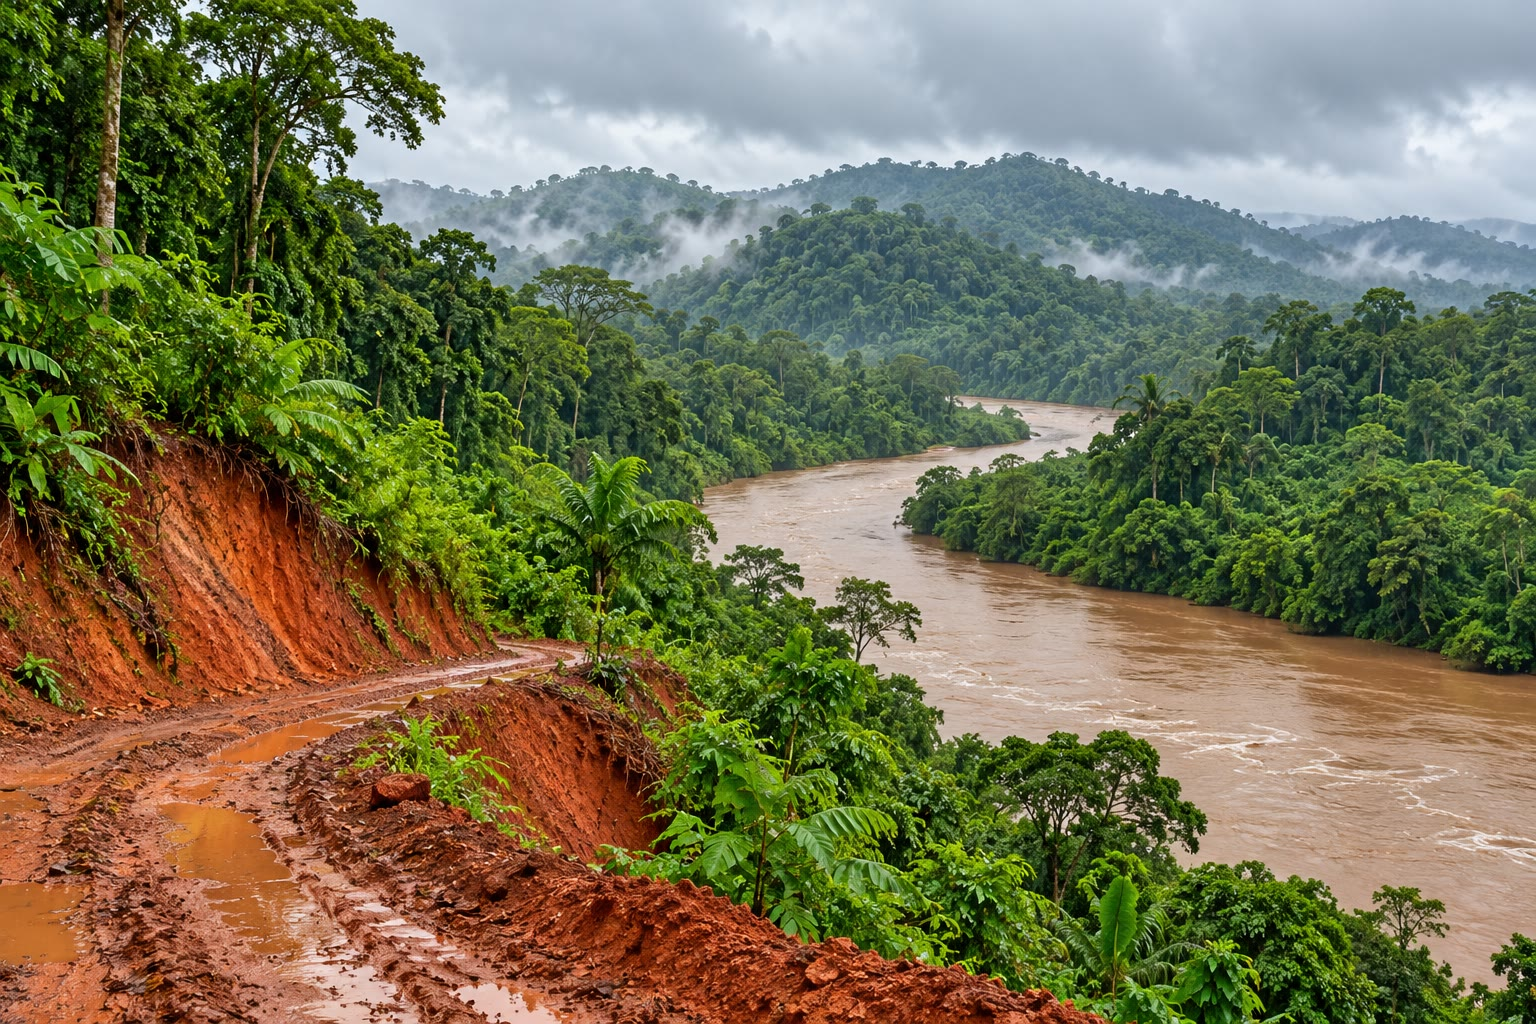
\includegraphics[width=0.66\linewidth]{images/book4/ai/b2-tropical-weathering.jpg}
\par\smallskip{\small 恒温器作用最强之处：炎热潮湿的低地，降雨落在
风化严重的红色土壤上，河流将风化产物带入海洋
（AI 生成插图）。}
\end{omfigure}

\section*{练习}\label{sec:b2:deep-time-climate:exercises}

除非另有说明，练习所用数据如下：工业化前大气中的碳
\qty{591}{PgC}（\qty{278}{ppm}）；$\qty{1}{Tmol}$ 的碳 $= \qty{0.012011}{PgC}$；硅酸盐
风化通量 $W_0 = \qty{0.138}{PgC.\text{年}^{-1}}$；海洋与
碳酸盐作用之后过剩量留在大气中的份额 $f = 0.08$；风化敏感度 $k_T = \qty{0.09}{K^{-1}}$；气候敏感度 $S =
\qty{3}{K}$；二氧化碳加倍的强迫 \qty{3.93}{W.m^{-2}}；$R =
\qty{8.314}{J.mol^{-1}.K^{-1}}$。
% ledger: ar6ch5:fig512, ipcc:erf-2xco2, derry24:fluxes, colbourn13:timescale, colbourn13:weathering, ipcc:ecs

\begin{exercise}[$\star$]\label{exo:b2:deep-time-climate:1}
工业化前，海洋表层储存了 \qty{900}{PgC}，中层与深层水体储存了 \num{37100}，
溶解有机碳为 700，生物体内为 3。
(a) 海洋共储存了多少碳？是大气的多少倍？(b) 将
\qty{3.5e6}{Tmol} 的表层库换算为拍克碳。(c) 其中多大比例位于
大气中？
\end{exercise}

\begin{exercise}[$\star$]\label{exo:b2:deep-time-climate:2}
利用\omterm{def:b2:deep-time-climate:carbon-cycle}{长期碳循环}图中的通量，取变质脱气为
\qty{3}{Tmol.\text{年}^{-1}}。(a) 将流入表层库的输入与输出相加。
(b) 火山、裂谷与\omterm{def:b2:metamorphic-facies:metamorphism}{变质作用}提供的输入占多大比例？(c) 利用输出项，求表层库中碳的
停留时间。
\end{exercise}

\begin{exercise}[$\star$]\label{exo:b2:deep-time-climate:3}
(a) 写出镁橄榄石 \ce{Mg2SiO4} 被二氧化碳和水风化、生成镁离子、碳酸氢根离子与溶解的
二氧化硅 \ce{SiO2} 的反应，并配平。(b) 镁随后以碳酸盐形式沉积，
写出净反应。(c) 需风化多少质量的镁橄榄石，
才能永久移除 \qty{1}{PgC}？（$M(\ce{Mg2SiO4}) = \qty{140.7}{g.mol^{-1}}$。）
\end{exercise}

\begin{exercise}[$\star$]\label{exo:b2:deep-time-climate:4}
按年代先后排列，注明各事件的时间，并对每一事件判断当时地球处于温室状态还是
冰室状态：早始新世气候最适期；赫南特期\omterm{def:b2:orbital-forcing:glacials}{冰期}；南极冰盖的
开始形成；图罗尼期；晚古生代冰川的最大范围；北半球冰盖的
主要扩张期；PETM。
\end{exercise}

\begin{exercise}[$\star\star$]\label{exo:b2:deep-time-climate:5}
(a) 验证活化能为 \qty{63}{kJ.mol^{-1}}、温度为 \qty{288}{K} 时能给出 $k_T =
\qty{0.09}{K^{-1}}$。(b) 对现场值 \qty{74}{kJ.mol^{-1}} 求 $k_T$。(c) 分别用两者求脱气增加
\qty{20}{\percent} 时的稳态升温。(d) 为什么气候敏感度
不参与 (c) 的计算？
\end{exercise}

\begin{exercise}[$\star\star$]\label{exo:b2:deep-time-climate:6}
将精确的阿伦尼乌斯因子 $\exp[-(E_{\text a}/R)(1/T - 1/T_0)]$ 与 $e^{k_T(T -
T_0)}$ 相比，其中 $k_T = E_{\text a}/(RT_0^2)$，取 $E_{\text a} = \qty{63}{kJ.mol^{-1}}$、$T_0 =
\qty{288}{K}$：(a) 在 $T = \qty{293}{K}$ 时；(b) 在 $T = \qty{318}{K}$ 时。(c) 证明近似因子与精确因子之比为
$\exp[E_{\text a}x^2/(RT_0^2(T_0 + x))]$，其中 $x = T - T_0$，
并求该比值达到 1.1 时的升温。
\end{exercise}

\begin{exercise}[$\star\star$]\label{exo:b2:deep-time-climate:7}
平滑后的汇编数据给出，在 \qty{419.5}{Ma} 时大气二氧化碳为 \qty{1444}{ppm}，而
记录末端为 \qty{276}{ppm}。(a) 求该下降过程的强迫。(b) 将其与
变亮的太阳所产生的 \qty{9}{W.m^{-2}} 相比较。(c) 求每百万年的平均下降速率（以 ppm 计），
并与拟合趋势的 \qty{3.4}{ppm} 相比较。两者为何可能不同？
\end{exercise}
% ledger: data:b4-foster2017, foster17:co2

\begin{exercise}[$\star\star$]\label{exo:b2:deep-time-climate:8}
(a) 将 \num{3000} 与 \qty{7000}{PgC} 分别分摊到 3 与
\qty{20}{ka} 内，由此得到怎样的释放速率范围？与 IPCC 所给出的每年 0.3 至 \qty{1.5}{PgC.\text{年}^{-1}} 相比较。(b) 2010 年人类排放
约为 \qty{35}{Gt} 的二氧化碳，换算为碳后进行比较。(c) 二氧化碳从 900 升至
\qty{2000}{ppm}。求强迫及 $S =
\qty{3}{K}$ 时的平衡升温，并与 PETM 前气候之上的 \qty{5}{\celsius} 升温相比较。
\end{exercise}
% ledger: ar6ch5:petm-release, usgs:volcanic-co2, ar6ch5:petm

\begin{exercise}[$\star\star$]\label{exo:b2:deep-time-climate:9}
山脉隆升使地球的风化能力 $W_0$ 增为原来的 1.2 倍，
脱气保持不变。(a) 求新的稳态温度变化。(b) 从
\qty{278}{ppm} 出发，求新的稳态二氧化碳浓度。(c) 在新的稳态下，硅酸盐风化速率与原来相比
是否不同？请说明理由。
\end{exercise}

\begin{exercise}[$\star\star\star$]\label{exo:b2:deep-time-climate:10}
(a) 用径流因子求恒温器的 e 折时间，取 $k = 0.09 + 0.65\times0.045$。
(b) 在数百万年尺度上，冰盖与植被也会作出响应；取地球系统敏感度为
每倍增 \qty{8}{K}（代替 $S$），求 $\tau$，并以 $k_T$ 计。(c) 这两种变化分别将
恒温器推向何方，以及 $E_{\text a}$ 与 $S$ 中哪一项的不确定性更为重要？
\end{exercise}

\begin{exercise}[$\star\star\star$]\label{exo:b2:deep-time-climate:11}
释放 \qty{5000}{PgC}（经海洋与碳酸盐作用之后）。(a) 求大气中的二氧化碳
浓度（以 ppm 计）与升温幅度。(b) 求初始净移除速率 $W - W_0$，以及
脉冲按该速率消失所需的时间。(c) 求线性化后移除 \qty{90}{\percent}
超出量所需的时间。(d) 若不作线性化而直接积分模型，则需 \qty{340}{ka}，为何更长？
\end{exercise}

\begin{exercise}[$\star\star\star$]\label{exo:b2:deep-time-climate:12}
(a) 在脱气量为 $V$、$C = C^*$ 的稳态附近线性化该模型，并证明
e 折时间为 $\tau' = A_0 (C^*/C_0)\ln 2/(f k S V)$。(b) 对脱气量升高
\qty{20}{\percent} 的稳态，求其值。(c) 在二氧化碳丰富的世界中，恒温器
更快还是更慢？为什么？
\end{exercise}

\begin{problem}[{周末问题——恒温器需要多长时间？}]\label{pb:b2:deep-time-climate:1}
本题根据实测通量构建恒温器的时间常数。数据取自
前述练习：洋脊、洋岛、岛弧与裂谷的脱气量依次为 \num{1.3}、\num{1.3}、4.5 和
\qty{4.2}{Tmol.\text{年}^{-1}}；硅酸盐风化量为 11 至 \qty{12}{Tmol.\text{年}^{-1}}；活化能
\qty{63}{kJ.mol^{-1}}（$T_0 = \qty{288}{K}$ 时）；大气质量为 \qty{5.1e18}{kg}，空气的平均
摩尔质量为 \qty{28.97}{g.mol^{-1}}。结果保留三位有效数字。

\noindent\textbf{第一部分——平衡。}
\begin{enumerate}
  \item 将火山与裂谷的脱气量相加，分别以 \unit{Tmol.\text{年}^{-1}} 和 \unit{PgC.\text{年}^{-1}} 计。
  \item 取 $W_0$ 为其取值范围的中值，并换算为 \unit{PgC.\text{年}^{-1}}。
  \item 比较两者。这一比较对\omterm{def:b2:deep-time-climate:carbon-cycle}{长期碳循环}说明了什么？
  \item 大气中含多少摩尔空气？\qty{591}{PgC} 的碳相当于多少摩尔，
        对应的\omterm{def:b2:atmospheric-thermodynamics:moist-air}{混合比}是多少？
  \item 若完全没有风化，第 1 小题中的脱气量需要多长时间才能
        向地表储库增加 \qty{591}{PgC}？
  \item 若其中比例 $f = 0.08$ 留在大气中，大气二氧化碳
        含量将升高为原来的几倍？
\end{enumerate}

\noindent\textbf{第二部分——线性化。}
\begin{enumerate}[resume]
  \item 由活化能求 $k_T$，并检验其四舍五入后是否为
        下文所用的 \qty{0.09}{K^{-1}}。
  \item 升温 \qty{1}{K} 时，风化速率增加为原来的几倍？
  \item 写出升温 $\Delta T$ 与超出量 $M$ 的关系式，并求其在 $M = 0$ 处的导数，
        单位为 \unit{K.PgC^{-1}}。
  \item 求 $W$ 对 $M$ 在 $M = 0$ 处的导数，单位为 \unit{\text{年}^{-1}}。
  \item 证明其倒数即为
        \cref{prop:b2:deep-time-climate:thermostat}中的时间常数 $\tau$。
  \item 在 $f$、$k$、$S$ 与 $W_0$ 中，哪些增大时会使恒温器变快？
\end{enumerate}

\noindent\textbf{第三部分——时间常数。}
\begin{enumerate}[resume]
  \item 求 $\tau$ 的数值。
  \item 取径流因子 $k = \qty{0.119}{K^{-1}}$，求其数值。
  \item 取 $k_T$ 及活化能 \qty{74}{kJ.mol^{-1}}，求其数值。
  \item 将这些结果与显式海洋模型给出的 \qty{200}{ka} 至 \qty{1}{Ma} 相比较。
  \item 新生代二氧化碳下降的 \qty{50}{Ma} 内可容纳多少个
        e 折时间？这说明下降期间碳循环处于什么状态？
  \item 若以每百万年 \qty{16}{ppm} 的速率变化，二氧化碳在一个 $\tau$ 内改变多少？
\end{enumerate}

\noindent\textbf{第四部分——相当于 PETM 规模的释放。}
\begin{enumerate}[resume]
  \item 释放 \qty{5000}{PgC}，经海洋与碳酸盐作用后，大气中残留的碳为多少，
        对应的二氧化碳浓度是多少 ppm？
  \item 求此时刻的升温幅度。
  \item 风化速率升高了多少？以 \unit{PgC.\text{年}^{-1}} 和百分比分别表示。
  \item 用线性化规律，超出量减少 \qty{90}{\percent} 需要多长时间？
  \item PETM 期间碳酸盐在约 \qty{100}{ka} 内恢复。试给出两点理由，说明
        真实地球可能比本模型恢复得更快。
  \item 总结：本模型中\omterm{def:b2:deep-time-climate:thermostat}{硅酸盐风化恒温器}的 e 折时间是多少？
\end{enumerate}
\end{problem}
% ledger: derry24:fluxes, colbourn13:weathering, colbourn13:timescale, ar6ch5:fig512, ar6ch5:petm, ar6ch5:cenozoic-co2, ipcc:ecs, earth:Matm, earth:Mmol
